%\part{Einfuehrung}

%----------------------------------------------------------------------------
\section{Vorraussetzungen}
\begin{frame}[fragile]
	\frametitle{Vorraussetzungen}
\huge Vorraussetzungen
\end{frame}

\begin{frame}
\frametitle{Ihre Erwartungen an die Veranstaltung}
	\begin{exampleblock}{Was m\"ochten Sie gerne behandeln?}
		\begin{itemize}
			 \item{}
			 \item{}
			 \item{}
			 \item{}
			 \item{}
		\end{itemize}
	\end{exampleblock}
\end{frame}

\begin{frame}
\frametitle{Erwartungen an die Veranstaltung}
	\begin{block}{Was sollten Sie am Ende k\"onnen?}
		\begin{itemize}
			 \item{Software Engineering als Teildisziplin der Informatik kennen}
			 \item{Grundpfeiler des Software Engineering kennen}
			 \item{Vorgehensmodelle der Softwareentwicklung beschreiben und abgrenzen}
			 \item{Softwarequalität messen und bewerten}
			 \item{Weiterf\"uhrende Konzepte verstehen und anwenden}
		\end{itemize}
	\end{block}
\end{frame}

%----------------------------------------------------------------------------
\section{Einführung}
\begin{frame}[fragile]
	\frametitle{Einführung}
\huge Einführung
\end{frame}

\begin{frame}[fragile]
	\frametitle{SW-Entwicklung im Studium}
	\begin{columns}
		\begin{column}{.5\textwidth}
			Aufgabe: Rekursives Take
			\newline\newline
			Implementieren Sie die Methode take(int n) die
			die ersten n Elemente eines Übergebenen Arrays
			vom Typ int als neues Array zurückgibt.
		\end{column}
		\begin{column}{.5\textwidth}
			\center
\includegraphics[width=1\textwidth,
			keepaspectratio=true]{bilder/student.png}
		\end{column}
	\end{columns}
\end{frame}

\begin{frame}
\frametitle{Die Realität}
	\begin{columns}
		\begin{column}{0.5\textwidth}
			\small
			\begin{itemize}
				\item Anforderungen mehrere 100 Seiten lang
				\item Anforderungen unklar, widersprüchlich, flexibel
				\item International verteilte Teams
				\item Mehrere tausend Nutzer in 5 Ländern
				\item Unterstützung von Chrome, Firefox, IE 6
				\item 6 Monate Projektlaufzeit, 500.000 LOC
			\end{itemize}
			\normalsize
		\end{column}
		\begin{column}{.5\textwidth}
			\center
\includegraphics[width=1\textwidth,
			keepaspectratio=true]{bilder/student_traurig.png}
		\end{column}
	\end{columns}
\end{frame}

\begin{frame}
\frametitle{Die Realität}
	Standish Group (http://www.standishgroup.com) veröffentlicht
	jährlich ``Chaos Report''.
	\newline\newline
	\begin{block}{Chaos Report 2015}
		\begin{itemize}
			\item 19\% der betrachteten IT-Projekte scheitern
			\item 52\% der betrachteten IT-Projekte drohen zu scheitern
			\item 29\% der betrachteten IT-Projekte sind erfolgreich
		\end{itemize}
	\end{block}
\end{frame}

\begin{frame}
\frametitle{Softwarekatastrophe ARIANE 5}
	\begin{quote}
		On June 4, 1996, on its maiden flight, the Ariane-5 was launched
		and performed perfectly for approximately 40 seconds. Then it began
		to veer off course. At the direction of the Ariane ground controller,
		the rocket was destroyed by remote control. \ldots total cost of the
		disaster was 500 million dollar.
	\end{quote}
	\begin{itemize}
		\item Flugbahn wird durch ``Inertial Reference System (SRI)'' gemessen,
		dessen Software teilweise von Ariane-4 übernommen wurde.
		\item Andere Flugbahndaten erzeugten Überlauf bei
		Konvertierung von 64-Bit Floating Point in 16-Bit Integer
		und verursachten Fehlfunktion des SRI-Systems.
	\end{itemize}
\end{frame}

\begin{frame}
\frametitle{Softwarekatastrophe Heartbleed}
	\begin{itemize}
		\item Heartbeat hält TLS-Verbindung am Leben
		\item Eine Seite schickt beliebig langen Payload, Gegenseite schickt die
		gleichen Daten wieder zurück
		\item Indikator für aufrechte Verbindung
	\end{itemize}
\end{frame}

\begin{frame}
\frametitle{Softwarekatastrophe Heartbleed}
	\center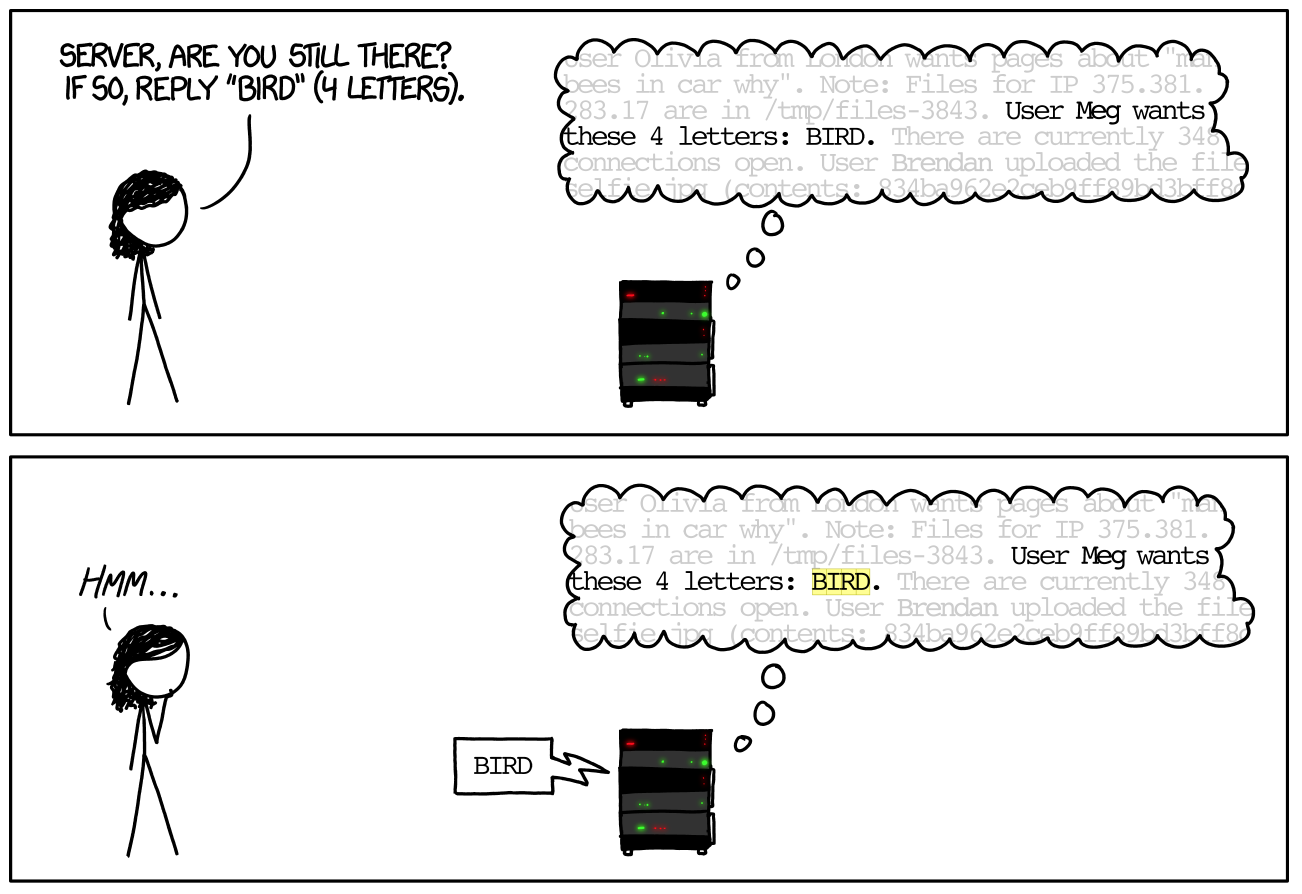
\includegraphics[width=1\textwidth,
	keepaspectratio=true]{bilder/heartbleed1.png}
\end{frame}

\begin{frame}
\frametitle{Softwarekatastrophe Heartbleed}
	\begin{itemize}
		\item Prüfung ob Payload der angegebenen Länge entspricht fehlte
		\item War der Payload kürzer als angegeben wurden Daten aus den darauffolgenden
		Speicherbereichen kopiert
		\item Da OpenSSL eine eigenen Speicherverwaltung implementiert waren diese Daten
		auch aus dem OpenSSL Kontext
	\end{itemize}
\end{frame}

\begin{frame}
\frametitle{Softwarekatastrophe Heartbleed}
	\center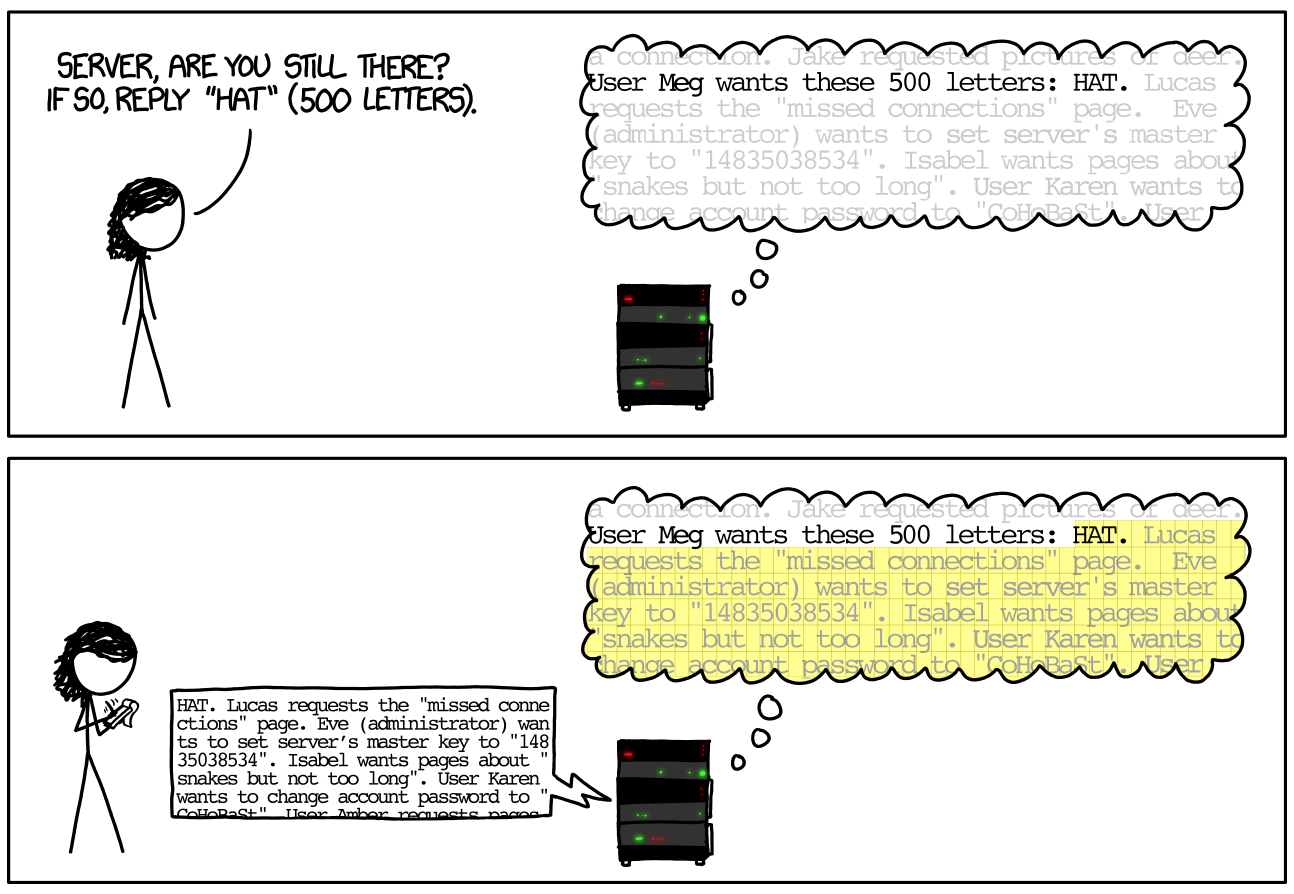
\includegraphics[width=1\textwidth,
	keepaspectratio=true]{bilder/heartbleed2.png}
\end{frame}

\begin{frame}
\frametitle{Softwarekrise}
	SW-Entwicklung in den 40er und 50er Jahren
	\small
	\begin{itemize}
		\item Teure Hardware
		\item Low-Level Programmierung (Assembler, fast kein OS)
		\item Von Experten bedient (Entwickler = Nutzer)
		\item numerisch-naturwissenschaftliche Probleme
	  	\item Codierung bekannter, mathematisch fundierter Algorithmen
	 	\item Viele Daten, einfache Algorithmen
		\item Häufig Batch-Systeme
		\item Fokus auf Effizienz
		\item Häufig ``Wegwerf-Software''
	\end{itemize}
	\normalsize
\end{frame}

\begin{frame}
\frametitle{Softwarekrise}
	SW-Entwicklung in den 60er Jahren bis heute
	\small
	\begin{itemize}
		\item Preiswerte Hardware mit viel Leistung
		\item Embedded Hardware die günstig ist und häufig eingesetzt wird
		\item Nicht-Informatiker nutzen die Software
		\item Vielzahl von Anwendungsbereichen
	  	\item Kritische Anwendungsbereiche wie Finanzsektor etc.
	  	\item Systeme sind komplex und interaktiv
		\item Software teurer als Hardware
		\item Lange Lebensdauer
	\end{itemize}
	\normalsize
\end{frame}

\begin{frame}
\frametitle{Softwarekrise}
	\begin{block}{Softwarekrise}
		\begin{itemize}
			 \item Programme werden immer komplexer
			 \item Passende Programmiersprachen, Methoden, Werkzeuge fehlen
		\end{itemize}
	\end{block}
	\begin{alertblock}{Folgen}
		\begin{itemize}
			 \item Kosten für Software steigen
			 \item Softwareprojekte scheitern
		\end{itemize}
	\end{alertblock}
	\begin{exampleblock}{Lösungsansatz}
		SW-Entwicklung als Ingenieurstätigkeit mit definiertem Vorgehen
		statt künstlerischer Tätigkeit
	\end{exampleblock}
\end{frame}

\begin{frame}
\frametitle{Softwarekrise}
	\begin{block}{Djikstra (The Humble Programmer)}
		\begin{quote}
			Als es noch keine Rechner gab, war auch das Programmieren noch kein
			Problem, als es ein paar leistungsschwache Rechner gab, war das
			Programmieren ein kleines Problem und nun, wo wir gigantische Rechner
			haben, ist das Programmieren zu einem gigantischen Problem geworden.
			In diesem Sinne hat die elektronische Industrie kein einziges Problem
			gelöst, sondern nur neue geschaffen. Sie hat das Problem geschaffen,
			ihre Produkte zu nutzen.
		\end{quote}
	\end{block}
\end{frame}

\begin{frame}
\frametitle{Was ist Software}
	\begin{block}{IEEE Definition}
		Software ist eine Sammlung von Computerprogrammen, Prozeduren, Regeln,
		zugehöriger Dokumentation und Daten
		\begin{itemize}
			 \item Programme sind eine Teilmenge von Software
			 \item SW beeinhaltet Dokumente die verschiedene Abstraktionsschichten
			 für verschiedene Zielgruppen beschreiben
		\end{itemize}
	\end{block}
\end{frame}

\begin{frame}
\frametitle{Probleme bei der Softwareentwicklung}
	\begin{itemize}
		 \item Kommunikationsprobleme mit Anwender
		 \item SW ist immateriell
		 \item SW ist leicht modifizierbar, Behebung von Fehlern wird unterschätzt
		 \item SW ist nur beobachtbar
		 \item Anforderungen ändern sich regelmäßig
		 \item SW altert über Umgebung ohne zu Verschleißen,
		 das führt zu immer neuen Erweiterungen und wachsender Komplexität
		 \item Verhalten für Software lässt sich nur schwer beweisen
		 \item \ldots
	\end{itemize}
\end{frame}

\begin{frame}
\frametitle{Software Engineering}
	\begin{itemize}
		\item Auslöser für Begriff ``Software Engineering'' war Softwarekrise von 1968
		\item Begriff ``Software Engineering'' wurde 1967 von F.L. Bauer (ehemaliger Prof. in München) 
		im Rahmen einer ``Study Group on Computer Science'' der NATO geprägt.
		\item Software wurde erstmals als Industrieprodukt bezeichnet
	\end{itemize}
\end{frame}

\begin{frame}
\frametitle{Was ist Software Engineering}
	\begin{block}{Definition IEEE}
		Software Engineering ist der systematische Ansatz für
		\begin{itemize}
			\item die Entwicklung,
			\item den Betrieb
			\item sowie die Wartung
		\end{itemize}
		von Software.
	\end{block}
\end{frame}

\begin{frame}
\frametitle{Was ist Software Engineering}
	\begin{block}{Definition Lehrbuch Software-Technick (Balzert) }
		Zielorientierte Bereitstellung und systematische Verwendung von Prinzipien, Methoden, Konzepten, 
		Notationen und Werkzeugen für die arbeitsteilige, ingenieurmäßige Entwicklung und Anwendung von 
		umfangreichen Software-Systemen. Zielorientiert bedeutet die Berücksichtigung z.B. von Kosten, 
		Zeit, Qualität.
	\end{block}
\end{frame}

\begin{frame}
\frametitle{Ziele des Software Engineerings}
	Effiziente Entwicklung von messbar qualitativ hochwertiger Software
	\small
	\begin{itemize}
		\item Korrektheit und Zuverlässigkeit
		\item Robustheit
		\item Effizienz
		\item Benutzerfreundlichkeit
		\item Wartbarkeit und Wiederverwendbarkeit
	\end{itemize}
	\normalsize
	\bigskip
	Qualitätsfaktoren
	\small
	\begin{itemize}
		\item Extern (für den Benutzer sichtbar)
		\item Intern (nur für den Entwickler sichtbar)
	\end{itemize}
	\normalsize
	\normalsize
\end{frame}

\begin{frame}
\frametitle{Phasen des Software Engineering}
Der systematische Ansatz im Software Engineering wird auch als
Entwicklungsprozess bezeichnet. Er beeinhaltet eine Reihe von Aktivitäten
die zur Entwicklung von Software führen.
\begin{itemize}
	\item Spezifikation
	\item Entwicklung
		\begin{itemize}
			\item Entwurf
			\item Implementierung
		\end{itemize}
	\item Validierung
	\item Evolution
		\begin{itemize}
			\item Weiterentwicklung
			\item Betrieb
		\end{itemize}
\end{itemize}
\end{frame}

\begin{frame}
\frametitle{Kleine Softwareprojekte}
	\begin{itemize}
		\item Wenige LOC
		\item SW für die eigene Verwendung
		\item Produkt spezifiziert sich selbst
		\item Lösung wird direkt entwickelt
		\item Validierung und Korrekturen am Endprodukt
		\item 1 Entwickler
		\item Komplexität gering
		\item Software besteht aus wenigen Komponenten
		\item Wenig bis keine Dokumentation nötig
		\item Keine Planung und Projektstruktur nötig
	\end{itemize}
\end{frame}

\begin{frame}
\frametitle{Große Softwareprojekte}
	\begin{itemize}
		\item Viele LOC
		\item SW für die Verwendung durch Dritte
		\item Klares Ziel, genaue Spezifikation erforderlich
		\item Lösung wird in Phasen entwickelt
		\item Tests in jeder Phase sind unerlässlich
		\item Produkt wird im Team entwickelt
		\item Hohe Komplexität macht Strukturierung der SW erforderlich
		\item Software besteht aus vielen Komponenten
		\item Dokumentation für den wirtschaftlichen Betrieb der SW erfoderlich
		\item Projektstruktur zwingend erforderlich
	\end{itemize}
\end{frame}

\begin{frame}
\frametitle{Wachstum des Kommunikationsbedarfs}
	\center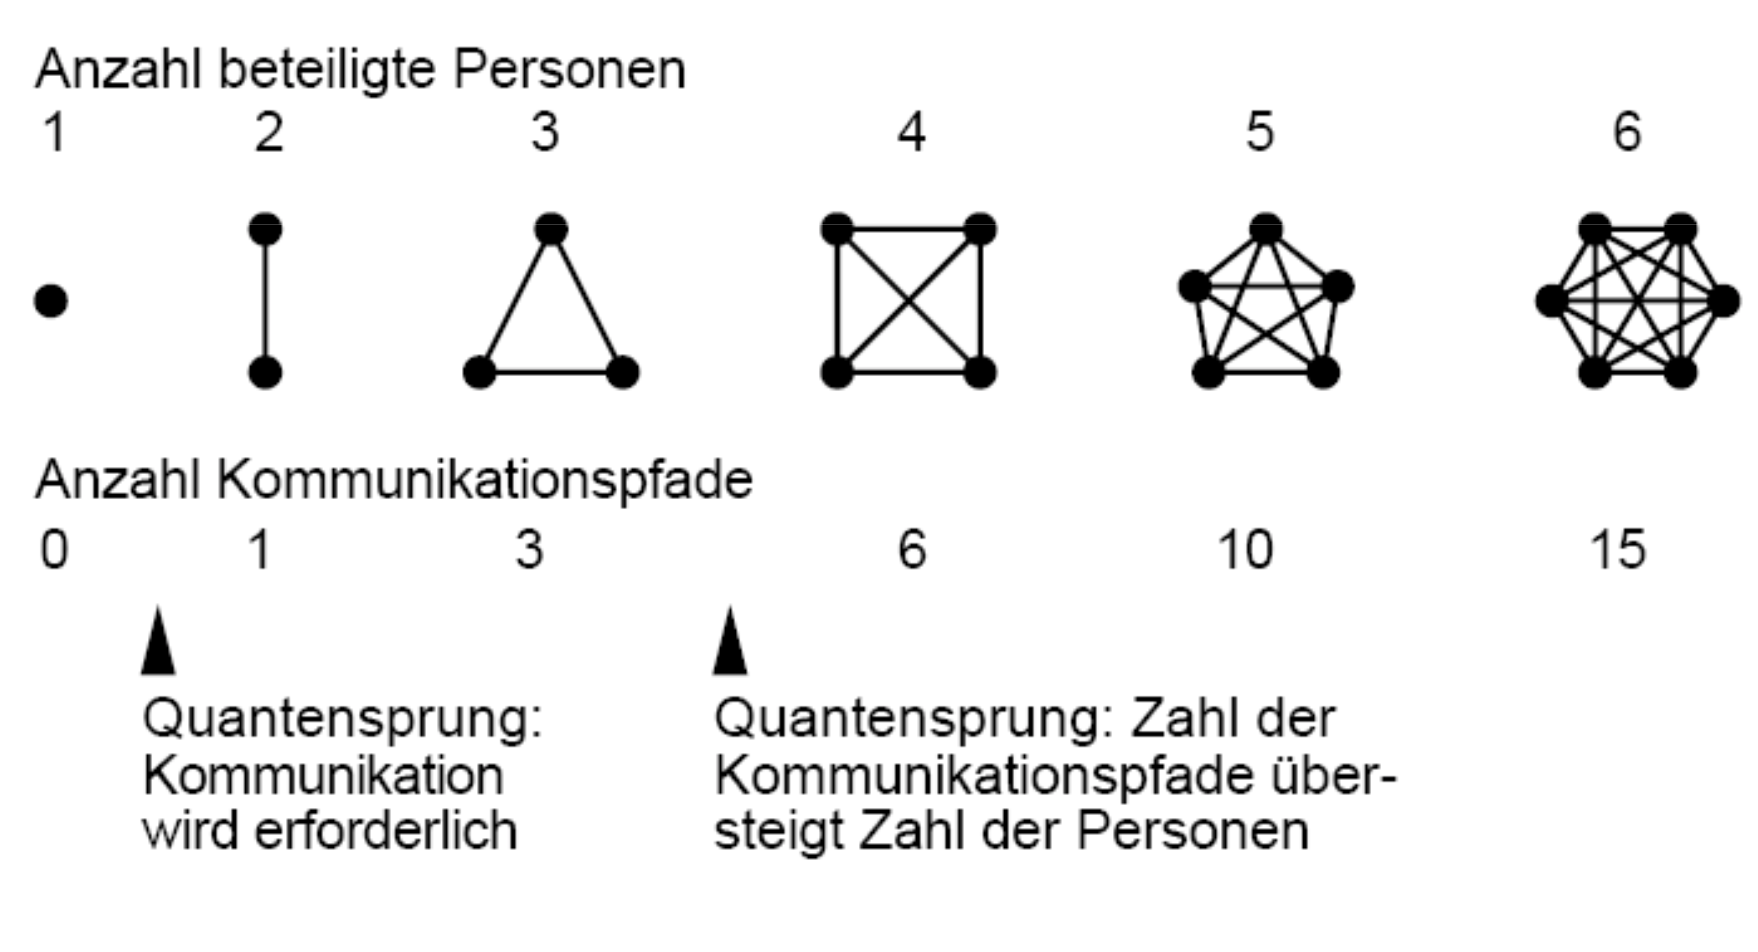
\includegraphics[width=1\textwidth,
	keepaspectratio=true]{bilder/kommunikationsbedarf.png}
\end{frame}

\begin{frame}
\frametitle{Wachstum des Aufwands}
	\center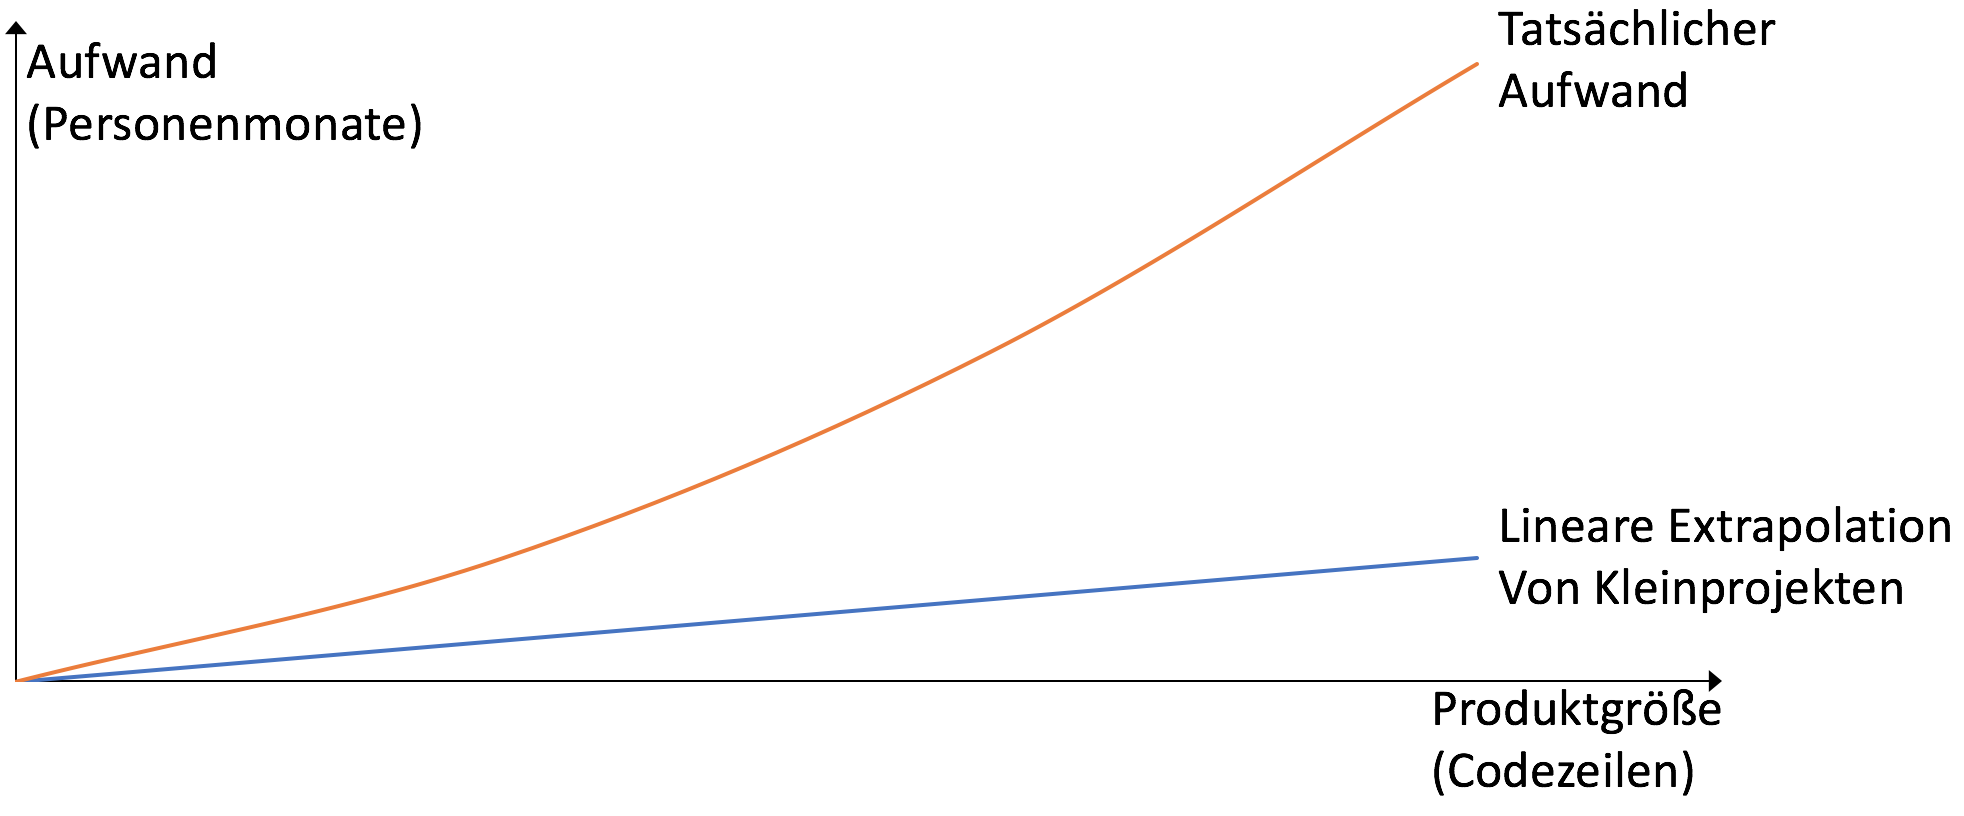
\includegraphics[width=1\textwidth,
	keepaspectratio=true]{bilder/projektaufwand.png}
\end{frame}

\begin{frame}
\frametitle{Aufwände aufgeschlüsselt}
	\center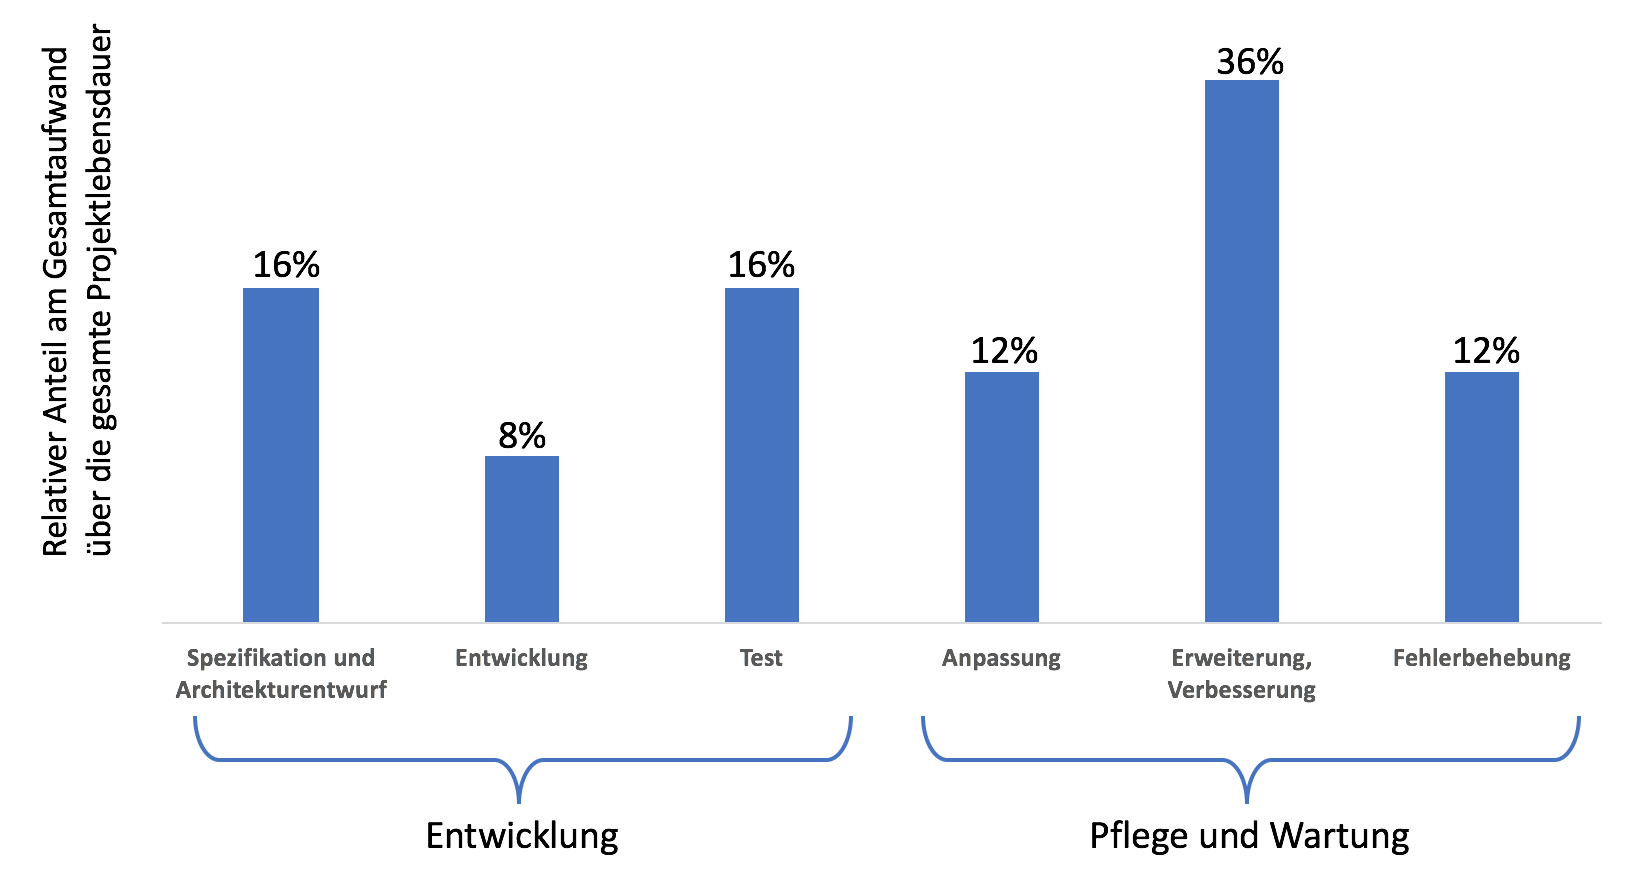
\includegraphics[width=1\textwidth,
	keepaspectratio=true]{bilder/anteil_aufwand.png}
\end{frame}

\begin{frame}
\frametitle{Übung 1.1}
	Eine Person braucht zum Bau einer 2m langen Bruecke 0,5 Tage. Wie lange brauchen 100 Leute für den Bau einer 2km langen Brücke?
	\begin{enumerate}
		\item Interpolieren Sie den Aufwand linear
		\item Warum ist die Berechnung aus Punkt 1 eine Milchmädchenrechnung?
	\end{enumerate}
\end{frame}

\ifloesung
\begin{frame}
\frametitle{Übung 1.1 - Lösung}
	Eine Person braucht zum Bau einer 2m langen Bruecke 0,5 Tage. Wie lange brauchen 100 Leute für den Bau einer 2km langen Brücke?
	\begin{enumerate}
		\item Aufwand = (2000m / 2m * 0.5PT) / 100 Personen = 5 Tage
		\item Mehr Kommunikation, Projekt deutlich Komplexer, Ressourcenbeschaffung, Logistik ...
	\end{enumerate}
\end{frame}
\fi

\begin{frame}
\frametitle{Übung 1.2}
	\scriptsize
	Eine Kundenbetreuerin im Firmenkundengeschäft einer Bank hat auf Grundlage eines 
	Tabellenkalkulationsprogramms eine kleine persönliche Anwendung geschrieben, 
	die sie bei der Überprüfung der Kredite der von ihr betreuten Firmen unterstützt. 
	Die notwendigen Daten gibt sie jeweils von Hand ein. Der Abteilungsleiter sieht 
	diese Anwendung zufällig, ist davon angetan und beschließt, sie allen Kundenbetreuerinnen 
	und -betreuer zur Verfügung stellen. Die notwendigen Daten sollen jetzt automatisch aus 
	den Datenbanken der Bank übernommen werden. Die Kundenbetreuerin gibt an, für die Entwicklung 
	ihrer Anwendung insgesamt etwa vier Arbeitstage aufgewendet zu haben. Der Abteilungsleiter 
	veranschlagt daher für die Übernahme und die gewünschten Änderungen einen Aufwand von einer 
	Arbeitswoche. Als die geänderte Anwendung endlich zur Zufriedenheit aller Beteiligten läuft, 
	sind jedoch rund acht Arbeitswochen Aufwand investiert. Der Abteilungsleiter erzählt die 
	Geschichte einem befreundeten Berater als Beispiel, dass Informatikprojekte nie ihre Termine 
	einhalten. Darauf meint der Berater trocken, der investierte Aufwand sei völlig realistisch 
	und normal. Begründen Sie warum.
	\normalsize
\end{frame}

\ifloesung
\begin{frame}
\frametitle{Übung 1.2 - Lösung}
	\scriptsize
	\begin{itemize}
		\item Die Kundenbetreuerin hat das Fachkonzept ihrer Tabellenkalkulationsanwendung vermutlich 
		schon vor den angegebenen vier Tagen Bearbeitungszeit im Kopf gehabt. Die Fremdentwickler 
		müssen dieses zumindest erst nachvollziehen.
		\item Die neue Anwendung ist durch die Datenbankanbindung mit den entsprechenden Schnittstellen 
		und Zugriffsrechteproblematiken deutlich komplexer.
		\item Der Kommunikationsaufwand schon allein von Kundenseite (viele Berater = viele unterschiedliche 
		Meinungen) ist erheblich
		\item Die neu entstandene ``professionelle'' Anwendung hat einen erheblich höheren Aufwand für 
		die Validierung als eine eigengenutzte Entwicklung.
		\item An die Bedienbarkeit (Nutzerschnittstelle) werden bei einer ``professionellen'' Anwendung 
		erheblich höhere Ansprüche gestellt.
	\end{itemize}
\end{frame}
\fi